\subsection{Benchmark Label Construction}

\paragraph{Metrics: Pairwise Preference as the Global Ranking Signal}
Rather than assigning absolute scores to individual images, we adopt a pairwise preference paradigm as the primary ranking signal: given two generated images $A$ and $B$ produced under the same prompt and reference set, the annotator is asked solely to determine which image is the better overall result, without assigning any numerical score to either candidate in isolation.

This design choice is motivated by two complementary considerations. First, absolute scoring in multi-subject personalized generation is inherently ill-defined: the space of possible failures is heterogeneous, and different annotators may apply inconsistent severity scales when mapping compositional defects to scalar values. Pairwise judgment sidesteps this calibration problem entirely, as relative comparisons are cognitively simpler and empirically more consistent across annotators. Second, pairwise preference naturally encodes graded severity information that cannot be captured by categorical labels alone. Two images may exhibit the same type of failure yet differ substantially in its degree; the preference signal resolves this ambiguity by reflecting which failure is more tolerable, providing a continuous severity proxy that complements the finer-grained diagnostic structure described below.

\paragraph{Metrics: Three Diagnostic Dimensions}
While pairwise preference captures overall quality ranking, it does not localize \textit{where} or \textit{why} a generated image fails. To provide this finer-grained diagnostic signal, we further decompose multi-subject failure into three orthogonal image-level dimensions:
\begin{itemize}
    \item \textbf{Existence}: whether all requested reference subjects are present without omission, cloning, or severe unidentifiable collapse.
    \item \textbf{Appearance}: whether the generated image preserves correct physical structure and local appearance for the requested reference subjects, without severe distortion or cross-subject feature bleeding.
    \item \textbf{Interaction}: whether subject-to-subject relations, actions, and prop assignments are aligned with the prompt.
\end{itemize}

For the three diagnostic dimensions, we adopt a softer aggregation strategy: in cases of disagreement, the final dimension score is computed as the average of the two annotations. For example, if annotator A assigns scores $(1, 1, 0)$ and annotator B assigns $(1, 0, 0)$ across the Existence, Appearance, and Interaction dimensions respectively, the resolved label is $(1, 0.5, 0)$. This asymmetric treatment reflects the differing roles of the two label types: the pairwise winner must be unambiguous to serve as a reliable ranking target, whereas fractional diagnostic scores naturally encode annotator uncertainty and provide a softer supervision signal during evaluation.

\paragraph{Training Label: MIB-Silver Label Generation with SOP-Guided LLMs Annotator}
\label{sec:method_sop_alignment}

Training our lightweight evaluator requires large-scale pairwise preference data. However, manually annotating our 60K-pair training set is prohibitively slow and expensive given the complex, multi-dimensional verification required for multi-subject generation. To overcome this bottleneck, we leverage MIB-Silver for training using frontier LLMs as scalable annotators, while strictly reserving human annotations for the MIB-Gold test set. To align machine and human judgments, we enforce a unified Standard Operating Procedure (SOP). By constraining both LLMs and humans to follow the exact same reasoning rubric, we ensure the silver training labels faithfully proxy the human decision-making process.

Unlike generic preference prompting, which often collapses into uninterpretable holistic judgments (e.g., favoring global aesthetics over prompt faithfulness), our SOP decomposes the pairwise comparison into a systematic, three-stage verification process: 1) \emph{Existence}: verifying the physical presence of all referenced subjects; 2) \emph{Appearance}: scrutinizing structural integrity and identity/wardrobe fidelity against the references; and 3) \emph{Interaction}: assessing the spatial arrangement and physical realism of the specified relations. Crucially, the SOP forces the judge to externalize its reasoning by generating a candidate-specific \emph{flaw log} before rendering a final binary preference. By explicitly penalizing missing entities, identity swapping, and interaction violations, this ``errors-first'' scaffolding acts as a regularizer, anchoring the LLM's latent preference policy to concrete compositional metrics rather than spurious visual correlations.

To further distill high-fidelity training signals and mitigate model-specific biases, we implement a cross-model consensus mechanism. We independently query two distinct frontier models (\texttt{gemini-2.5-flash} and \texttt{gemini-3.1-flash-lite-preview}) using the identical SOP. We then construct the final training set by taking the intersection of their predictions, retaining only the pairwise comparisons where both models yield the exact same preference. While this intersection rule reduces the total yield, it acts as a rigorous precision filter, effectively pruning examples where preference is driven by idiosyncratic model noise or ambiguous image quality. The resulting high-agreement subset provides a robust, conservative proxy for human preference. The exact prompt used to enforce this SOP in our pipeline is reproduced in Appendix~\ref{sec:app_SOP}. It explicitly separates independent candidate scoring from the final pairwise decision, defines strict edge cases, and mandates a JSON schema that forces the LLM to articulate flaws before concluding.


\paragraph{Testing Label: MIB-Gold Label Generation with Human Double-Blind Annotation}
To construct a high-quality gold test set, all labels are collected exclusively from human annotators following a double-blind protocol: each image pair is independently reviewed by two annotators without knowledge of each other's judgments.

The gold set covers \textbf{1{,}260 prompts} evaluated across \textbf{4 generative models}, yielding 2 pairwise comparisons per prompt and resulting in 2{,}520 unique image pairs. Under the double-blind protocol, each pair is annotated independently by two human judges, bringing the total annotation workload to \textbf{5{,}040 individual annotation tasks}.

For the global ranking signal, we require strict consensus: if the two annotators disagree on the pairwise winner, the sample is considered ambiguous and discarded from the gold set. For the three diagnostic dimensions, disagreements are resolved by averaging the two scores, naturally encoding annotator uncertainty as a soft supervision signal.






\subsection{MIB Construction}
\begin{figure}
    \centering
    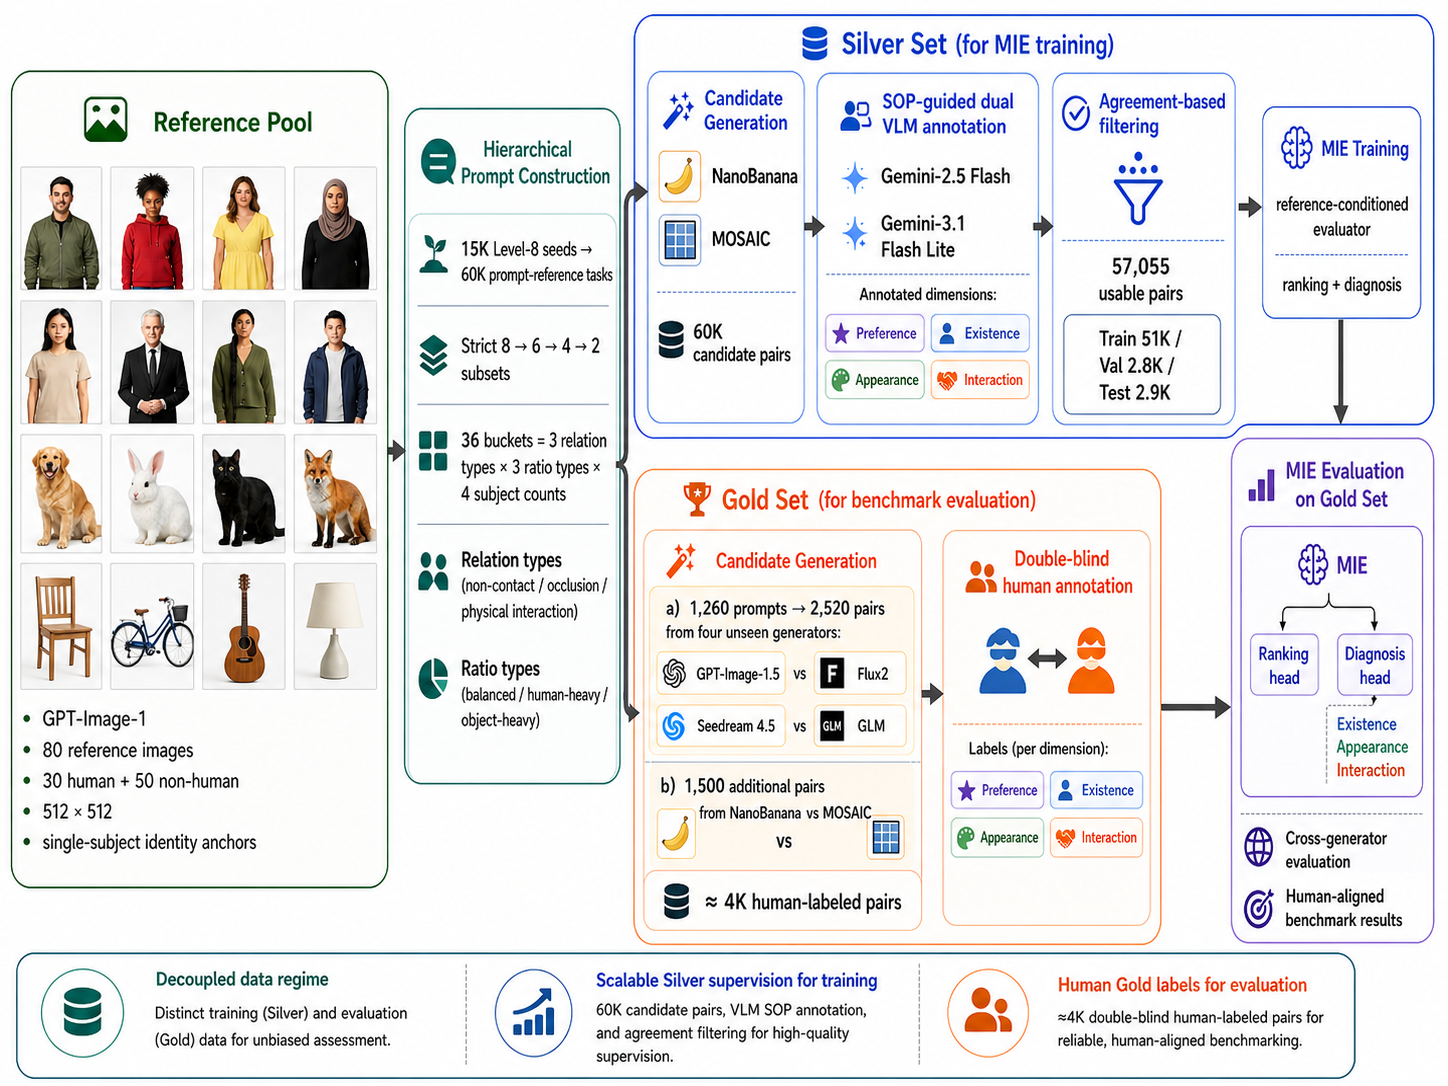
\includegraphics[width=1\linewidth]{mibe_overview.png}
    \caption{Overview of MIBE. The framework decouples reference construction, hierarchical prompt construction, candidate generation, and label acquisition. The Silver Set provides scalable SOP-guided VLM supervision for training MIE, while the Gold Set is double-blind human-labeled and reserved for benchmark evaluation.}
\label{fig:mibe_construction}
    \label{fig:placeholder}
\end{figure}
MIB is the data substrate of MIBE. It consists of controlled prompt-reference tasks, paired generated candidates, and their associated preference and diagnostic labels. Each task specifies a guiding prompt, a set of reference subjects, and two candidate generations produced under the same prompt-reference condition, enabling controlled comparison across subject counts, relation types, and generator outputs.

MIB follows a decoupled data regime that separates reference construction, prompt-task design, candidate generation, and label acquisition into independent stages. Reference images are constructed as single-subject identity anchors, while candidate images are generated as multi-subject interaction scenes under controlled prompt-reference conditions. This design allows subject identity, scene complexity, relation type, candidate generator, and annotation source to be controlled separately, reducing confounding factors in benchmark construction and enabling a clean separation between scalable evaluator training and human-centered benchmark evaluation.


We construct 60K prompt-reference tasks from 15K hierarchical seeds, where each seed produces four related prompts with $N \in \{8,6,4,2\}$ subjects. Each family starts from an eight-subject scene and is reduced into six-, four-, and two-subject variants by removing entities and their associated relations. This hierarchical decomposition ensures that the core scene semantics remain invariant across complexity levels. Consequently, observed performance degradation can be more directly attributed to the increased density of entity-relation constraints rather than tangential shifts in prompt distribution.

\subsubsection{Prompt Construction}
\begin{figure}
    \centering
    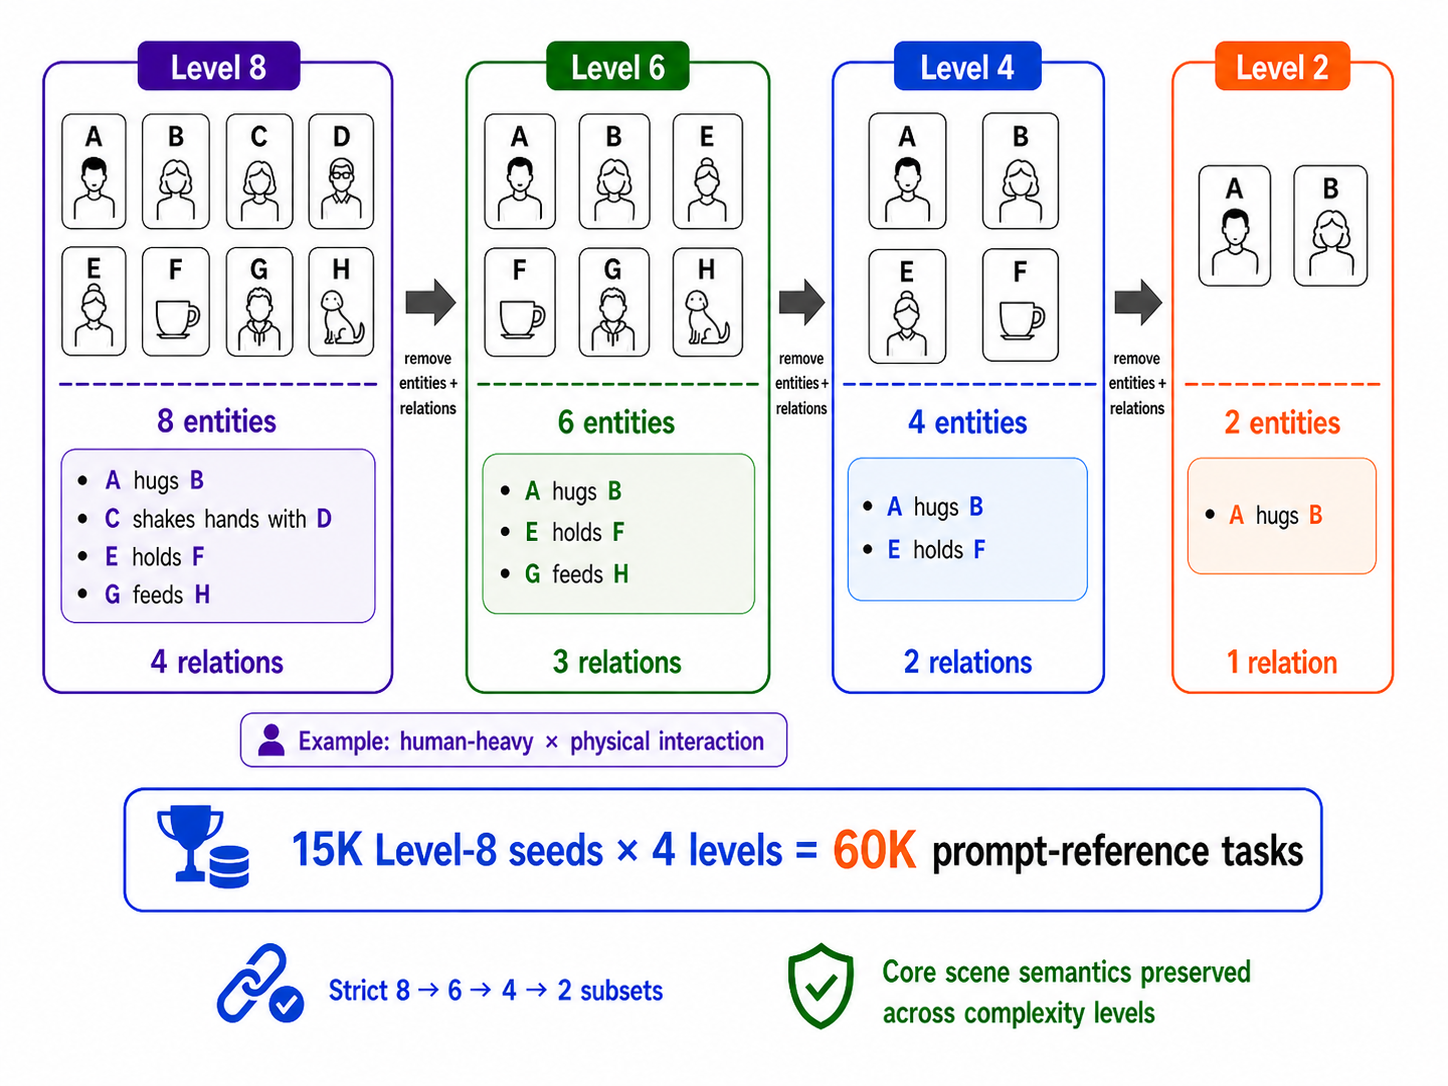
\includegraphics[width=0.5\linewidth]{hierarchical_prompt_construction.png}
    \caption{Hierarchical prompt construction. Each Level-8 seed is reduced into strict Level-6, Level-4, and Level-2 subsets by removing entities and their associated relations, preserving core scene semantics while varying entity-relation density.}
    \label{fig:placeholder}
\end{figure}


The prompt space is factorized by subject count, human/object composition, and relation type, yielding $3 \times 3 \times 4 = 36$ buckets. Human/object composition includes balanced, human-heavy, and object-heavy configurations, with exact human/non-human counts specified in Table~\ref{tab:entity_ratio_levels}. Prompts are distributed approximately uniformly across the 36 buckets.

\begin{table}[t]
\centering
\small
\begin{tabular}{lcccc}
\toprule
\textbf{Ratio Type} & \textbf{Level 8} & \textbf{Level 6} & \textbf{Level 4} & \textbf{Level 2} \\
\midrule
Balanced
& 4H, 4N
& 3H, 3N
& 2H, 2N
& 1H, 1N \\

Human-heavy
& 6H, 2N
& 4H, 2N
& 3H, 1N
& 2H, 0N \\

Object-heavy
& 2H, 6N
& 2H, 4N
& 1H, 3N
& 0H, 2N \\
\bottomrule
\end{tabular}
\caption{Human/non-human composition for each ratio type and scene complexity level. H denotes human entities, and N denotes non-human entities.}
\label{tab:entity_ratio_levels}
\end{table}

Relation type is organized into three broad categories: non-contact relations, occlusion relations, and physical interaction relations. We use separate template sets for the three categories to reduce boundary leakage during prompt generation. Non-contact relations include spatial or perceptual relations such as standing beside, facing, or looking at another subject. Occlusion relations describe partial visibility constraints without active engagement, such as one subject standing behind or partially blocking another subject. Physical interaction relations include both direct subject-to-subject interactions, such as hugging, petting, or shaking hands, and object-mediated interactions, such as holding or feeding.

Because relation types can overlap in natural scenes, we assign each task to the most restrictive applicable category, following the priority order: physical interaction $>$ occlusion $>$ non-contact. For each bucket, we also specify the participant structure of core relations, such as human-human, human-object, or object-object relations. Relations are assigned at the highest complexity level and then reduced together with the corresponding entities for lower-complexity prompts. To keep relation assignment interpretable, each entity participates in at most one core relation within a prompt.

All prompts are grounded in a white-studio setting with a global scale constraint. Specifically, each English prompt is prepended with: ``White studio. Keep all entities at realistic scale.'' This reduces background, lighting, layout, and unrealistic scale confounders, such as small objects being rendered at implausibly large sizes.

We apply automatic consistency checks using a rule-based parser and a lightweight LLM validator. These checks verify that assigned entities are explicitly mentioned, unassigned entities are excluded, human/non-human counts match the target bucket, lower-complexity prompts remain strict subsets of higher-complexity prompts, duplicate prompts are removed, the same entity is not reused as the subject of multiple independent relation statements, and interaction-specific keywords are not introduced into non-contact prompts.

\subsubsection{Reference Image Generation}

MIB uses a fixed pool of 80 reference subjects, including 30 human references and 50 non-human references. Human references cover diverse age groups, gender presentations, ethnicities, clothing styles, hairstyles, and visual appearances. Non-human references include animals, furniture, tools, wearable items, and common manipulable objects. This mixture allows MIB to evaluate both person-person binding and person-object or object-object binding under multi-subject personalized generation.

All reference images are generated using GPT-Image-1 and standardized as single-subject studio images at $512 \times 512$ resolution. Each reference image is produced as an isolated identity anchor, without multi-subject interactions or scene-specific relational context. The fixed reference pool allows the same subjects to be recombined across different prompts, making comparisons across complexity levels and relation types more controlled.


\subsubsection{Multi-subject Personalized Image Generation}

For each prompt-reference task, a personalized image generator receives a guiding prompt together with the corresponding reference images as visual conditioning inputs, and produces a candidate image. In our benchmark, reference subjects are provided as image-level identity anchors rather than as fine-tuned LoRA weights, ensuring a unified inference interface across generators. MIB constructs paired comparisons by placing two candidate generations under the same prompt-reference condition. This pairwise design controls for the prompt and reference set, so that annotators and evaluators compare only the relative quality of the two generated outputs.

For the Silver Set, we generate 60K candidate pairs using NanoBanana and MOSAIC. These two generators are selected because preliminary inspection shows complementary failure modes, including identity loss, subject omission, appearance leakage, and relation hallucination. This contrast creates informative pairwise supervision across existence, appearance, and interaction dimensions. Importantly, the reference images are generated separately using GPT-Image-1, so neither silver candidate generator is advantaged by sharing the same generation process as the reference pool. This separation reduces generator-specific leakage and makes the silver supervision less tied to the visual prior of either candidate generator.

For the Gold Set, we construct approximately 4K human-labeled candidate pairs. The Gold Set contains two subsets. First, for 1,260 main prompts, we generate candidate images using four state-of-the-art generators: GPT-Image-1.5, Flux2, Seedream 4.5, and GLM. For each prompt, we construct two pairwise comparisons: GPT-Image-1.5 versus Flux2, and Seedream 4.5 versus GLM, yielding 2,520 main-generator pairs. Rather than exhaustively comparing all six model pairs, we use two fixed cross-model matchups to balance comparison diversity and annotation cost. Second, we include 1,500 additional NanoBanana-versus-MOSAIC pairs to evaluate performance on seen-generator pairs under human annotation. For all Gold Set comparisons, both candidates are conditioned on the same reference images and guiding prompt, so the pairwise labels measure relative generation quality under an identical prompt-reference condition. Candidate order is randomized as Image A or Image B before annotation. Before labeling, we remove missing, corrupted, or blank generations through automatic validity checks.




\begin{table}[t]
\centering
\small
\begin{tabular}{p{0.24\linewidth}p{0.34\linewidth}p{0.34\linewidth}}
\toprule
\textbf{Attribute} & \textbf{Silver Set} & \textbf{Gold Set} \\
\midrule
Purpose 
& MIE training 
& Human benchmark evaluation \\

Prompt-reference tasks 
& 60,000 
& 1,260 main prompts + 1,500 additional prompts \\

Prompt construction 
& \multicolumn{2}{p{0.72\linewidth}}{15K Level-8 seeds $\times$ 4 complexity levels, with strict $8 \rightarrow 6 \rightarrow 4 \rightarrow 2$ hierarchical subsets} \\

Candidate generators 
& NanoBanana, MOSAIC 
& GPT-Image-1.5, Flux2, Seedream 4.5, GLM; plus NanoBanana and MOSAIC for additional seen-generator evaluation \\

Candidate pair construction 
& NanoBanana vs. MOSAIC for each prompt-reference task 
& GPT-Image-1.5 vs. Flux2 and Seedream 4.5 vs. GLM for each main prompt; NanoBanana vs. MOSAIC for additional prompts \\

Candidate pairs 
& 60,000 
& 4,020 total pairs: 2,520 main-generator pairs + 1,500 NanoBanana/MOSAIC pairs \\

Annotation source 
& SOP-guided dual VLM consensus 
& Double-blind human annotation \\

Annotators 
& Gemini-2.5-Flash and Gemini-3.1-Flash-Lite 
& Two independent human annotators per pair \\

Label types 
& Pairwise preference; Existence; Appearance; Interaction 
& Pairwise preference; Existence; Appearance; Interaction \\

Usable pairs 
& 57,055 
& 4,020 human-labeled pairs \\

Evaluation role 
& Train 51K / Val 2.8K / Test 2.9K 
& Seen-generator evaluation: 1,500 pairs; unseen-generator evaluation: 2,520 pairs \\
\bottomrule
\end{tabular}
\caption{Dataset statistics for MIB. The Silver Set provides scalable SOP-guided VLM supervision for training MIE, while the Gold Set is fully human-labeled under a double-blind protocol. The Gold Set contains both seen-generator pairs from NanoBanana/MOSAIC and unseen-generator pairs from GPT-Image-1.5, Flux2, Seedream 4.5, and GLM.}
\label{tab:dataset_statistics}
\end{table}



\subsubsection{Label Construction}

MIB provides two complementary forms of supervision: pairwise preference labels for global ranking and diagnostic labels for failure localization. Pairwise preference captures which candidate is better overall under the same prompt-reference condition, while diagnostic labels identify whether each candidate fails in subject existence, reference appearance preservation, or interaction grounding.

\paragraph{Pairwise preference.}
Rather than assigning absolute scores to individual images, we adopt pairwise preference as the primary global ranking signal. Given two generated images $A$ and $B$ produced under the same prompt and reference set, the annotator determines which image is the better overall result, without assigning a numerical score to either candidate in isolation.

This design is motivated by two considerations. First, absolute scoring in multi-subject personalized generation is difficult to calibrate: the failure space is heterogeneous, and different annotators may apply inconsistent severity scales when mapping compositional defects to scalar values. Pairwise judgment reduces this calibration burden by asking for a relative comparison under a shared prompt-reference condition. Second, pairwise preference captures graded severity information that categorical labels alone cannot represent. Two images may exhibit the same type of failure yet differ substantially in degree; the preference signal resolves this ambiguity by indicating which failure is more tolerable.

\paragraph{Diagnostic labels.}
While pairwise preference captures overall quality ranking, it does not localize where or why a generated image fails. We therefore decompose multi-subject generation quality into three complementary diagnostic dimensions:
\begin{itemize}
    \item \textbf{Existence}: whether all requested reference subjects are present without omission, duplication, or severe unidentifiable collapse.
    \item \textbf{Appearance}: whether the generated image preserves the physical structure and local appearance of the requested reference subjects, without severe distortion or cross-subject feature bleeding.
    \item \textbf{Interaction}: whether subject-to-subject relations, actions, and object assignments are aligned with the prompt.
\end{itemize}

For diagnostic labels, we adopt a soft aggregation strategy. In cases of annotator disagreement, the final dimension score is computed as the average of the two annotations. For example, if annotator A assigns scores $(1, 1, 0)$ and annotator B assigns $(1, 0, 0)$ across Existence, Appearance, and Interaction, respectively, the resolved label is $(1, 0.5, 0)$. This treatment reflects the different roles of the two label types: the pairwise winner must be unambiguous to serve as a reliable ranking target, whereas fractional diagnostic scores encode annotator uncertainty and provide softer supervision for evaluator training and analysis.

\paragraph{MIB-Silver annotation with SOP-guided VLM judges.}
Training MIE requires large-scale pairwise preference and diagnostic supervision. However, manually annotating 60K image pairs is prohibitively slow and expensive given the multi-dimensional verification required for multi-subject personalized generation. We therefore construct MIB-Silver using SOP-guided frontier VLM judges, while reserving human annotations exclusively for MIB-Gold.

To align scalable machine annotation with the intended human evaluation protocol, we use a unified Standard Operating Procedure (SOP) for both VLM and human annotators. The SOP decomposes each comparison into a three-stage verification process: 1) \emph{Existence}, verifying the physical presence of all referenced subjects; 2) \emph{Appearance}, checking structural integrity and identity or appearance fidelity against the references; and 3) \emph{Interaction}, assessing whether spatial relations, physical interactions, and object assignments follow the prompt.

Unlike generic preference prompting, which can collapse into uninterpretable holistic judgments or over-weight global aesthetics, our SOP requires the judge to produce candidate-specific flaw logs before rendering a final preference decision. This errors-first structure encourages the judge to ground its decision in concrete compositional failures, such as missing entities, identity swaps, appearance leakage, and interaction violations.

To further improve label precision and mitigate model-specific annotation bias, we use a cross-model consensus mechanism. We independently query two frontier VLMs, \texttt{gemini-2.5-flash} and \texttt{gemini-3.1-flash-lite-preview}, using the identical SOP. We retain only the comparisons for which both models produce the same pairwise preference. Although this intersection rule reduces total yield, it acts as a conservative precision filter by pruning examples where preference may be driven by ambiguous image quality or idiosyncratic model behavior. The resulting high-agreement subset serves as scalable training supervision for MIE, and its effectiveness is validated against the human-annotated Gold Set. The exact SOP prompt is reproduced in Appendix~\ref{sec:app_SOP}.

\paragraph{MIB-Gold annotation with double-blind human evaluation.}
To construct a high-quality human evaluation set, we collect MIB-Gold labels exclusively from human annotators following a double-blind protocol. Each image pair is independently reviewed by two annotators, without either annotator knowing the other's judgment or the identity of the generators that produced the images.

MIB-Gold contains approximately 4K human-labeled pairs. It includes 2,520 unseen-generator pairs from 1,260 prompts, where each prompt yields two comparisons among GPT-Image-1.5, Flux2, Seedream 4.5, and GLM, and 1,500 additional seen-generator pairs generated by NanoBanana and MOSAIC. Under the double-blind protocol, each pair is annotated independently by two human judges.

For the global ranking signal, we require strict consensus: if the two annotators disagree on the pairwise winner, the sample is considered ambiguous and excluded from the final preference-evaluation subset. For the three diagnostic dimensions, disagreements are resolved by averaging the two annotations, naturally encoding annotator uncertainty as a soft diagnostic signal.
